\preamble{Verb}{Verbs In English}
\chapter{Overview}
Verbs are words that express an action or a state of being. The main verb of a sentence is usually found at the beginning and followed by the subject, while auxiliary verbs are used to complete various tenses.\\\\
\textbf{For example:} He went home early after he was done with work.\\
The main verb here is “went” because it is the verb that carries most of the meaning. “Was” is an auxiliary verb because it helps make the tense of the sentence past tense.\\\\
Verbs have different forms depending on how or where they appear in a sentence:
\begin{itemize}
    \item Regular Verbs
    \item Irregular Verbs
    \item Transitive Verbs
    \item Intransitive Verbs
    \item Finite Verbs
    \item Infinite Verbs
    \item Action Verbs
    \item Helping Verbs
    \item Linking Verbs
\end{itemize}

\chapter{Types Of Verbs}
\section{Regular Verbs}
A regular verb is a verb that forms its past tense and past participle by adding -ed to the base form of the verb.\\\\
\textbf{For example,} the regular verb walk becomes walked.\\
Regular verbs are one of three main types of verbs in English. The other two types are irregular verbs and modal verbs. Irregular verbs do not follow the pattern of adding -ed to form their past tense and past participle. Modal verbs are a special type of verb that is used to express ability, permission, or obligation.

\section{Irregular Verbs}
Irregular verbs are verbs that don’t follow the normal rules for conjugating verbs in English. For example, the verb “to be” is irregular because it doesn’t change form when you add different pronouns (I am, you are, he/she/it is).\\
ESL students often have trouble learning irregular verbs because they don’t have a set pattern to follow. However, with enough practice and memorization, most students can eventually learn all of the irregular verbs in English. There are many verb lists and exercises available online to help ESL students master this topic.


\newpage
\section{Transitive Verbs}
A transitive verb is a verb that requires an object.\\ 
\textbf{For example:} I eat an apple. The apple is the object of the verb “eat.”\\\\
ESL students often have difficulty using transitive verbs correctly because many English verbs can be used both transitively and intransitively, depending on the context.\\
\textbf{For example,} the verb “to sleep” can be used either intransitively (I sleep) or transitively (I sleep in a bed). It’s important for ESL students to learn which verbs are typically used transitively and which are typically used intransitively.

\section{Intransitive Verbs}
Intransitive verbs are a type of verb that does not require a direct object to complete its meaning.\\
\textbf{For example,} the intransitive verb “to sleep” does not require a direct object to be complete, as in “I slept for eight hours last night.”\\\\
ESL students can find intransitive verbs difficult because they do not always follow the same rules as transitive verbs. In particular, they do not always have an obvious subject and object. For this reason, it is important for ESL students to learn how to identify intransitive verbs and understand their meanings. This will help them to produce accurate sentences in English and improve their language skills overall.

\newpage
\section{Finite Verbs}
A finite verb is a verb that has a specific tense and number, and it appears as the main verb in a sentence. 
In English, there are three finite verb forms: the present tense, the past tense, and the future tense.\\
\textbf{For example:}
\begin{itemize}
    \item I am writing a report. (present tense)
    \item I wrote a report yesterday. (past tense)
    \item I will write a report tomorrow. (future tense)
\end{itemize}

\section{Infinite Verbs}
ESL students might be wondering what “infinite verbs” are. 
In English grammar, there are two types of verbs: finite and infinite. 
Finite verbs are those that have a specific number of forms, whereas infinite verbs don’t have a specific number of forms. 
They simply go on and on… Hence the name “infinite”.\\\\
Some common examples of infinite verbs are: to love, to know, to be etc. 
These verbs can keep going for ever because there’s no set form that they have to take. 
As long as you continue speaking in the present or past tense, the verb will keep going on and on. There’s no limit to how long it can keep going!

\newpage
\section{Action Verbs}
Action verbs express physical or mental actions. 
They are often used to describe what a person is doing. 
Some common action verbs are run, walk, eat, and play.\\\\
When describing what they are doing, they can use these verbs to make their sentences more interesting and accurate. \\
\textbf{For example,} a student might say “I am writing a paper,” instead of “I write a paper.”\\
Action verbs can also make writing more exciting for ESL students. 
By using powerful action words, students can create scenes that come alive on the page.

\section{Helping Verbs}
Helping verbs, also known as auxiliary verbs, are used to create compound verb tenses or to express nuances in the meaning of a verb. 
In English, there are three main helping verbs: be, do, and have.\\\\
Be is used to indicate the tense of a sentence (present, past, future), to form the passive voice, and to create reflexive verbs.\\
Do is used as an imperative (command) verb and to form questions and negatives.\\
Have is used to form perfect verb tenses and to indicate possession.

\newpage
\section{Liking Verbs}
A linking verb is a type of verb that connects the subject of a sentence with a word or phrase that describes or identifies the subject. In other words, a linking verb links the subject to either an adjective or a noun.\\
Some common linking verbs are: be, become, feel, grow, look, seem, smell, sound, and taste.\\
Linking verbs are often used in questions to test if someone knows English grammar well.\\\\
\textbf{For example:} “He is very smart.” versus “He seems very smart.” The first sentence uses the linking verb “is” to connect the subject “he” with the adjective “smart”. The second sentence uses the linking verb “seems” to connect the subject “he”.

\chapter{Infographics}
\graphicspath{{D:/Projects/English-Project/project-folders/Verb}}
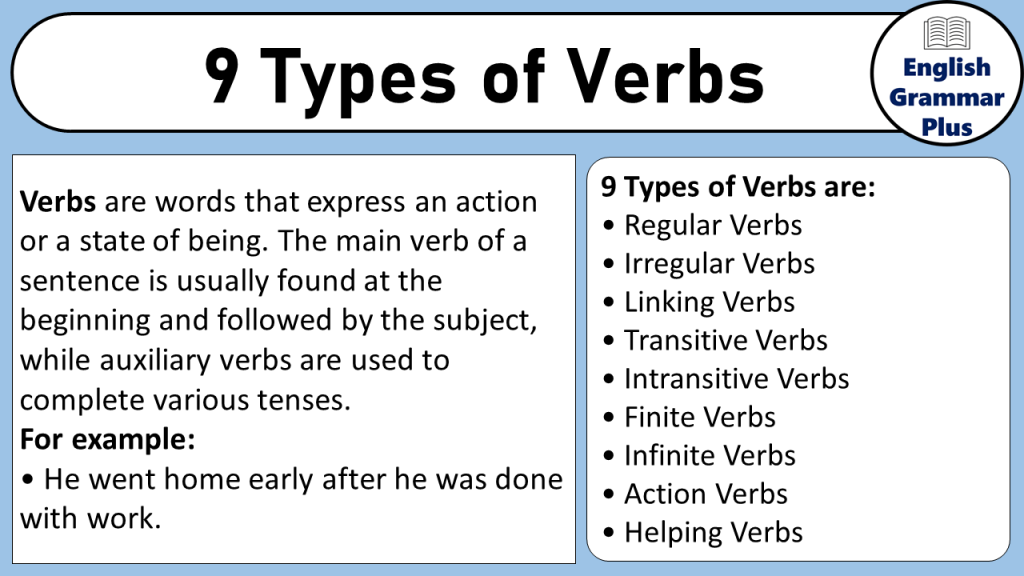
\includegraphics[scale=0.25]{overview.png}
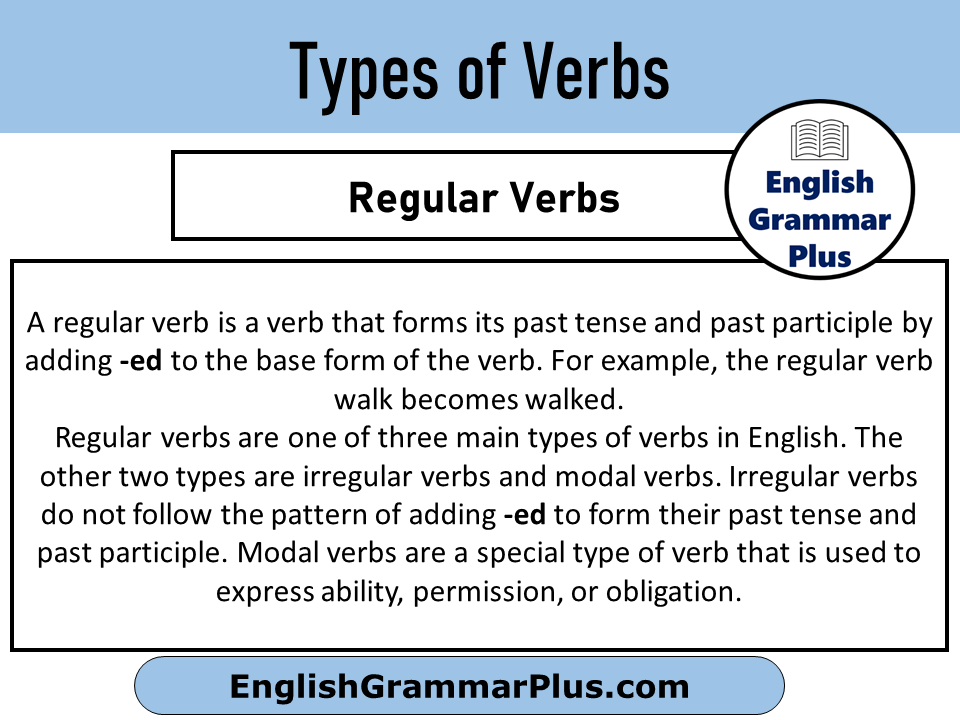
\includegraphics[scale=0.25]{regularVerbs.png}
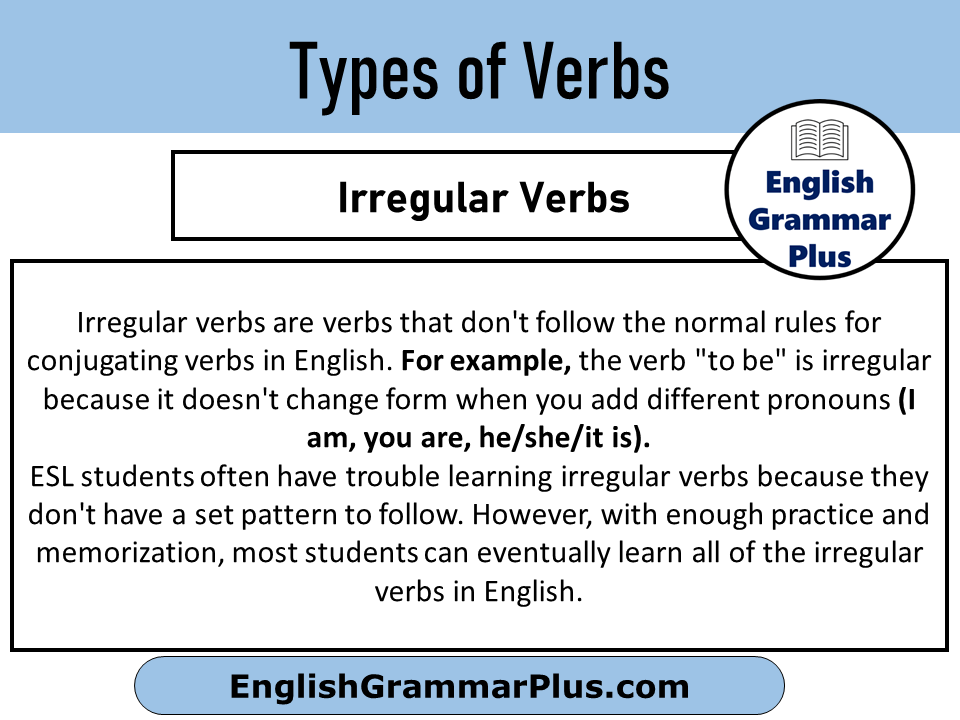
\includegraphics[scale=0.25]{irregularVerbs.png}
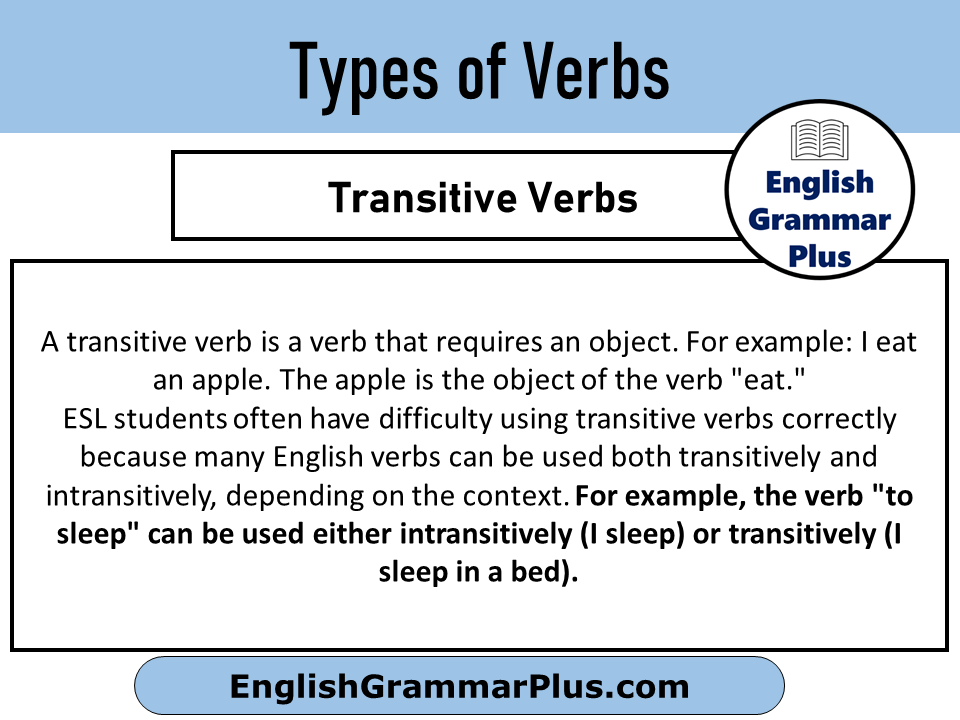
\includegraphics[scale=0.25]{transitiveVerbs.png}
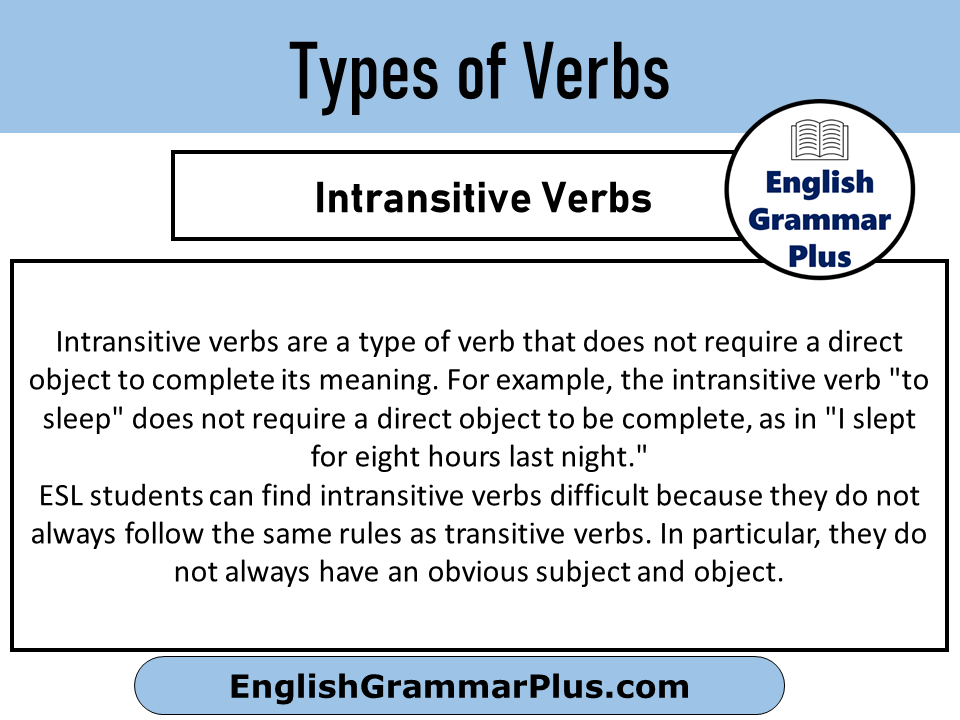
\includegraphics[scale=0.25]{intransitiveVerbs.png}
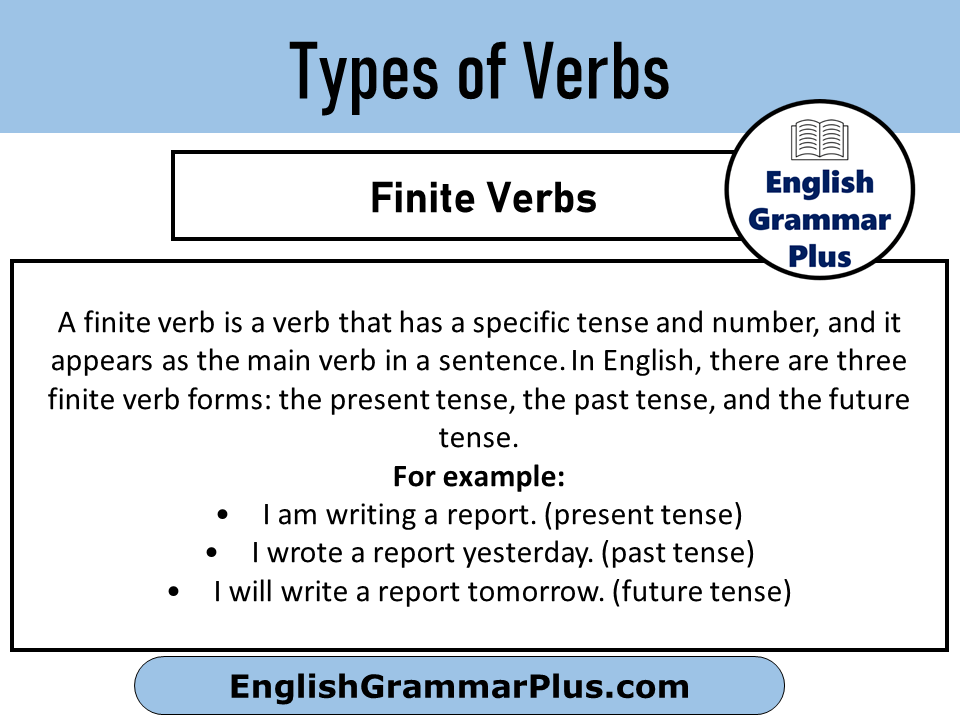
\includegraphics[scale=0.25]{finiteVerbs.png}
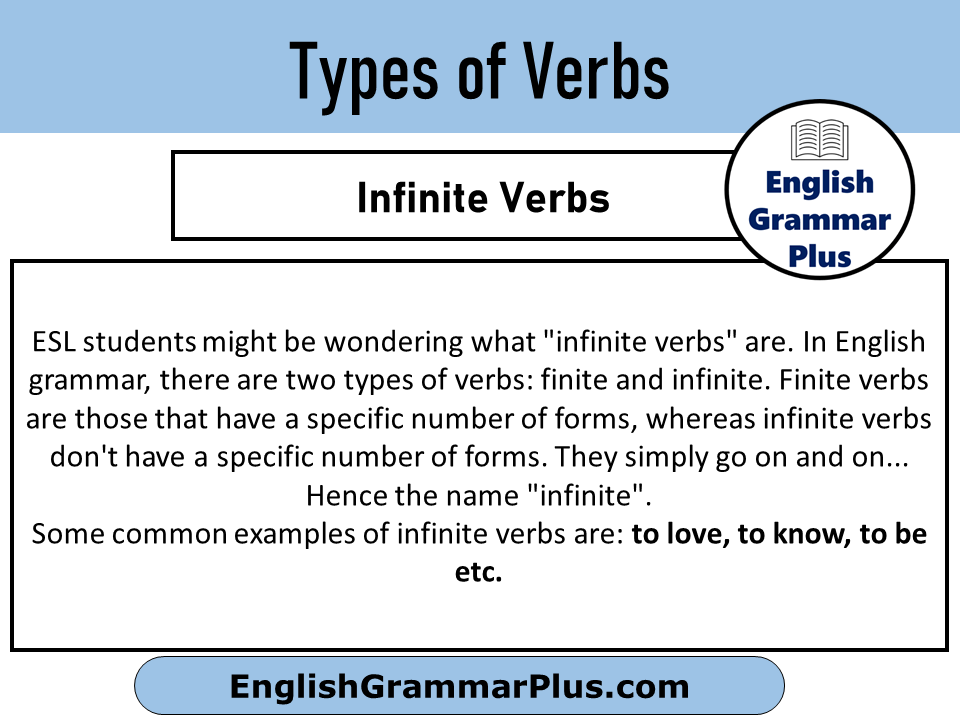
\includegraphics[scale=0.25]{infiniteVerbs.png}
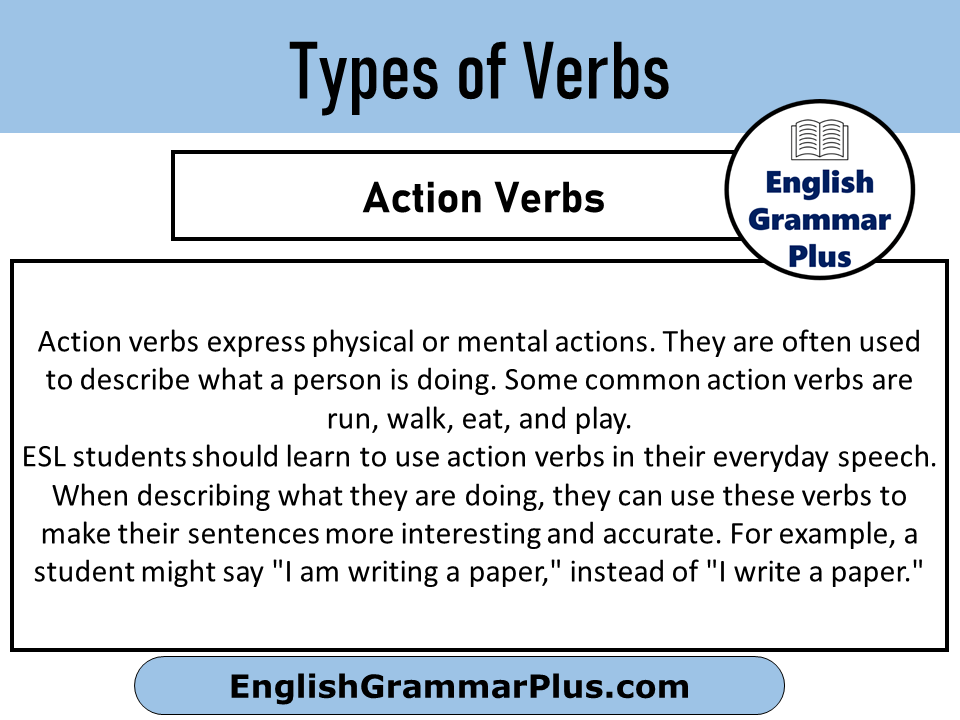
\includegraphics[scale=0.25]{actionVerbs.png}
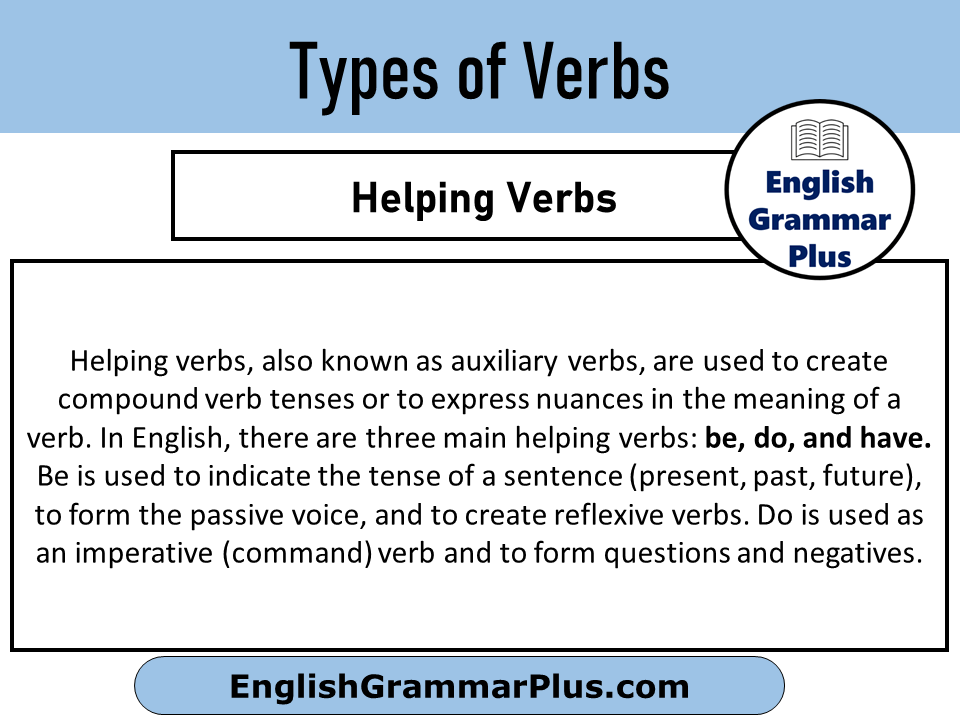
\includegraphics[scale=0.25]{helpingVerbs.png}
\includegraphics[scale=0.25]{likingVerbs.png}